\documentclass[a4paper,12pt]{article}
\usepackage{amsmath}
\usepackage{amssymb}
\usepackage[polish]{babel}
\usepackage{polski}
\usepackage[utf8]{inputenc}
\usepackage{indentfirst}
\usepackage{geometry}
\usepackage{array}
\usepackage[pdftex]{color,graphicx}
\usepackage{subfigure}
\usepackage{afterpage}
\usepackage{setspace}
\usepackage{color}
\usepackage{wrapfig}
\usepackage{listings}
\usepackage{datetime}

\renewcommand{\onehalfspacing}{\setstretch{1.6}}

\geometry{tmargin=2.5cm,bmargin=2.5cm,lmargin=2.5cm,rmargin=2.5cm}
\setlength{\parindent}{1cm}
\setlength{\parskip}{0mm}

\newenvironment{lista}{
\begin{itemize}
  \setlength{\itemsep}{1pt}
  \setlength{\parskip}{0pt}
  \setlength{\parsep}{0pt}
}{\end{itemize}}

\newcommand{\linia}{\rule{\linewidth}{0.4mm}}

\definecolor{lbcolor}{rgb}{0.95,0.95,0.95}
\lstset{
    backgroundcolor=\color{lbcolor},
    tabsize=4,
  language=C++,
  captionpos=b,
  tabsize=3,
  frame=lines,
  numbers=left,
  numberstyle=\tiny,
  numbersep=5pt,
  breaklines=true,
  showstringspaces=false,
  basicstyle=\footnotesize,
  identifierstyle=\color{magenta},
  keywordstyle=\color[rgb]{0,0,1},
  commentstyle=\color{green},
  stringstyle=\color{red}
  }

\begin{document}

\noindent
\begin{tabular}{|c|p{11cm}|c|} \hline 
Grupa 6 & Dariusz Szczupak, Kamil Wanat & \ddmmyyyydate\today \tabularnewline
\hline 
\end{tabular}


\section*{Zadanie 4 - Liczby Pierwsze MPI}

Zadanie laboratoryjne polegało na zaimplementowaniu programu sprawdzającego czy podane liczby są liczbami pierwszymi, czy złożonymi. Program w swoim działaniu wykorzystuje MPI(Message Passing Interface) - standard przesyłania komunikatów pomiędzy procesami, w celu jego zrównoleglenia. Problem został rozwiązany przy pomocy algorytmu ''naiwnego". Jest to metoda nieco wolniesza niż metody probabilistyczne, jednak dająca zdecydowanie lepsze wyniki. Polega ona na dzieleniu testowanego elementu przez kolejne liczby od 2 do pierwiastka kwadratowego z tejże. W naszym programie podejście naiwne zostało nieco zmodyfikowane. Zamiast sprawdzać dzielniki od 2 do pierwiastka z każdej liczby, znajdujemy najpierw liczbę maksymalną, a następnie testujemy wszystkie liczby przy pomocy dzielnikow od 2 do sqrt(max). Ponadto nie testujemy każdej liczby osobno dla danego dzielnika, lecz cały zbiór. 

\begin{lstlisting}
for (int i = 1; i < size; i++) {   
            if (i == (size - 1))             
                end = tab.size();
            vector <number> templateTable(tab.begin() + begin, tab.begin() + end);       
            begin = end;                                                                 
            end += step;

            uint tableSize = templateTable.size();                                       
            MPI_Send(&tableSize, 1, MPI_INT, i, 0, comm);                               
            MPI_Send(&sqr, 1, MPI_INT, i, 1, comm);                                     
            MPI_Send(templateTable.data(), tableSize, myType, i, 2, comm);              
        }
        vector <number> tab2;         
        vector <number> concatTable;
for (int i = 1; i < size; i++) {    

            MPI_Recv(&d, 1, MPI_INT, i, 0, comm, MPI_STATUS_IGNORE);                    
            tab2.resize(d);                                                             
            MPI_Recv(tab2.data(), d, myType, i, 1, comm, MPI_STATUS_IGNORE);            
            concatTable.insert(concatTable.end(), tab2.begin(), tab2.end());            
        }
\end{lstlisting}


Powyższy kod źródłowy przedstawia działanie zasadniczej części procesu zerowego (głównego). Jego zadaniem jest podział całego wektora liczb pierwszych na mniejsze podzbiory, a następnie ich rozesłanie do procesów o numerze rank wiekszym niż 0. Odpowedzialna jest za to pierwsza pętla for. Zakres liczb które wchodzą w skład danego podzbioru ustalają zmienne begin oraz end a ich ilość zmienna step. Wycięcie zbioru danych wykonywane jest w konstruktorze wektora templateTable. Do procesów potomnych wysyłane sa trzy wiadomości: pierwsza z rozmiarem wektora danych, druga z wartością pierwiastka do którego testujemy liczby oraz trzecia z danymi zawartymi w wektorze.
Kolejną częścią programu jest odebranie oraz sklejenie danych z wektorem wynikowym. Program główny oczekuje na odebranie od procesów potomnych dwóch wiadomości: pierwsza z rozmiarem danych oraz druga z dynymi właściwymi zapisanymi do wektora tab2. Następnie dane te są doklejane za pomocą funkcji insert do wektora wynikowego - concatTable.
Aby możliwe było wysyłanie wektora który zawiera w sobie typ złożony, musieliśmy zarejestrować taki typ w programie. Sposób rejestracji nowego typu MPI przedstawiony jest na poniższym listingu. 

\begin{lstlisting}
 int lengths[2] = {1, 1};                                                 // ilosc zmiennych w strukturze
    MPI_Aint offsets[2] = {offsetof(number, value), offsetof(number, prime)};  // przesuniecie bitowe zmiennych struktury
    MPI_Datatype types[2] = {MPI_LONG,MPI::BOOL};                           // podstawowe typy skladajace sie na nasz typ
    MPI_Datatype myType;                                                    // deklaracja nowego typu
    MPI_Type_create_struct(2, lengths, offsets, types, &myType);            // utworzenie nowego typu
    MPI_Type_commit(&myType);
\end{lstlisting}


\begin{figure}[!hbp]
	\centering
  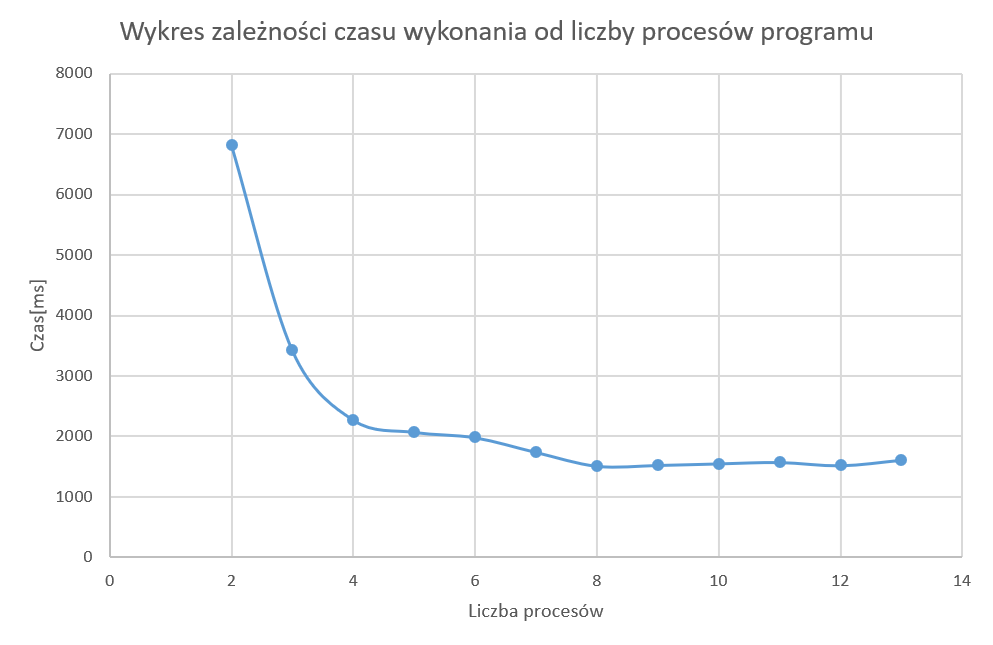
\includegraphics[width=0.7\textwidth]{wykres.png}
  \caption{Wykres zależności czasu wykonywania od liczby procesów}
\end{figure}
Powyższy wykres przedstawia zależność czasu wykonywania się programu od liczby procesów z jaką został on uruchomiony. Wykres rozpoczyna sie od 2 procesów, ponieważ proces zerowy wykorzystywany jest jedynie do podziału zbioru na mniejsze części, wysłanie danych do procesów oraz ich odebranie i sklejenie. Wobec tego nie jest możliwe uruchomienie programu z parametrem n=1. Jak dobrze widać na wykresie czas nie zmniejsza się liniowo wraz ze wzrostem liczby wątków. Spowodowane jest to wzrostem czasu obliczeń dla procesu zerowego ze względu na większą ilość operacji komunikacji pomiędzy procesem zerowym a procesami potomnymi. Każda z takich operacji zajmuje pewną ilość czasu, tak więc im więcej procesów uruchomimy, tym większy stanie się czas wykonywania operacji wysyłania/odbierania danych. Podobnie jak w przypadku OpenMP najlepszy wynik uzyskujemy dla 8 procesów (tyle ile wątków dostarcza serwer CUDA). Późniejsze zwiększanie ilości procesów zwiększa nam nieznacznie czas wykonania obliczeń. Również tak jak w poprzednich zadaniach widoczny jest pewien moment w którym czas obliczeń jest na stałym poziomie, a następnie znów się zmniejsza. Taka sytuacja występuje dla 6 procesów. Powodowane jest to prawdopodobnie zwiększeniem narzutu na procesor przez większą liczbę komunikatów oraz włączeniem oraz architekturą sewera CUDA (8 wątków przy 4 fizycznych rdzeniach z wykorzystaniem technologii HyperThreading). 

\begin{wrapfigure}{r}{0.5\textwidth}
  \vspace{-20pt}
  \begin{center}
  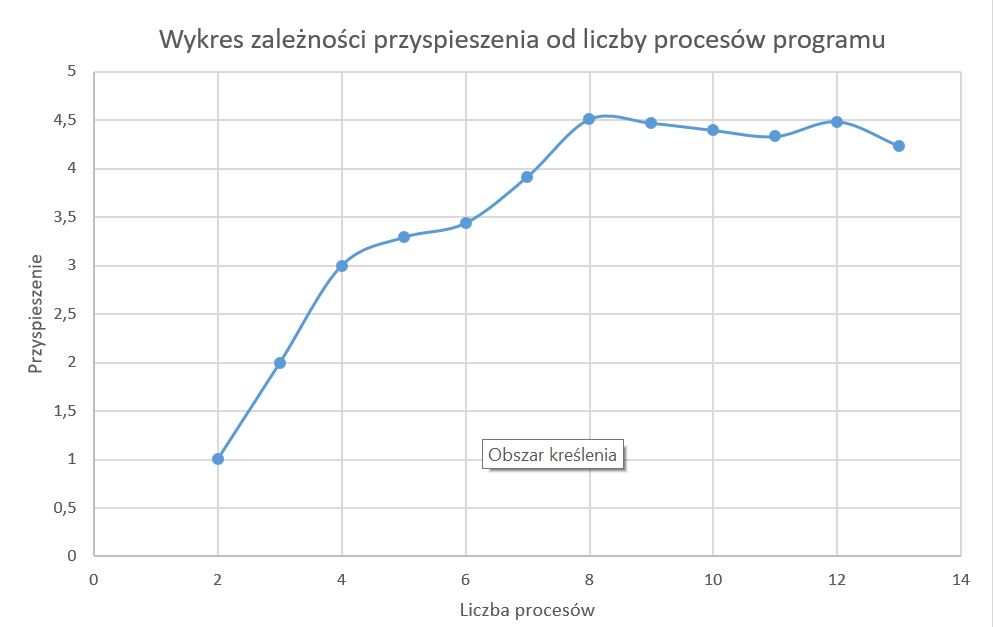
\includegraphics[width=0.45\textwidth]{wykres1.png}
  \end{center}
  \vspace{-20pt}
  \caption{Wykres przyspieszenia}
  \vspace{-10pt}
\end{wrapfigure}


Wykres przyspieszenia programu testującego liczby pierwsze pokazuje czy i jak udało się zrównoleglić działanie programu. Z tego wykresu możemy wyciągnąć analogiczne wnioski do tych, które zostały opisane pod wykresem zależności czasu wykonania od ilości wątków procesora. Tutaj również widać spadek przyspieszenia od liczby procesów - 5 wzwyż oraz wzrost czasu obliczeń dla liczby procesów powyżej 8. 
 
Dane przeprowadzanych testów:
\begin{lista}
 \item Wzięto pod uwagę średnią pomiarów czasów wykonania programu dla liczby wątków z przedziału od 2 do 13. 
 Program był uruchamiany dla pliku pobranego z internetu.
 \item Do mierzenia czasu wykorzystano MPIWtime.
 \item Testy zostały wykonane na serwerze cuda.iti.pk.edu.pl . 
 \item W czasie testów na serwerze zalogowany był jedynie użytkownik testujący.
\end{lista}


\end{document}

